\documentclass[tikz]{standalone}
\usepackage[utf8]{inputenc}

\usetikzlibrary{shapes.geometric, arrows}

\tikzstyle{startstop} = [rectangle, rounded corners, minimum width=3cm, minimum height=1cm,text centered, draw=black, fill=red!30]
\tikzstyle{io} = [trapezium, trapezium left angle=70, trapezium right angle=110, minimum width=3cm, minimum height=1cm, text centered, draw=black, fill=blue!30]
\tikzstyle{process} = [rectangle, minimum width=3cm, minimum height=1cm, text centered, text width=3cm, draw=black, fill=orange!30]
\tikzstyle{decision} = [diamond, minimum width=3cm, minimum height=1cm, text centered, draw=black, fill=green!30]
\tikzstyle{arrow} = [thick,-latex]

\begin{document}

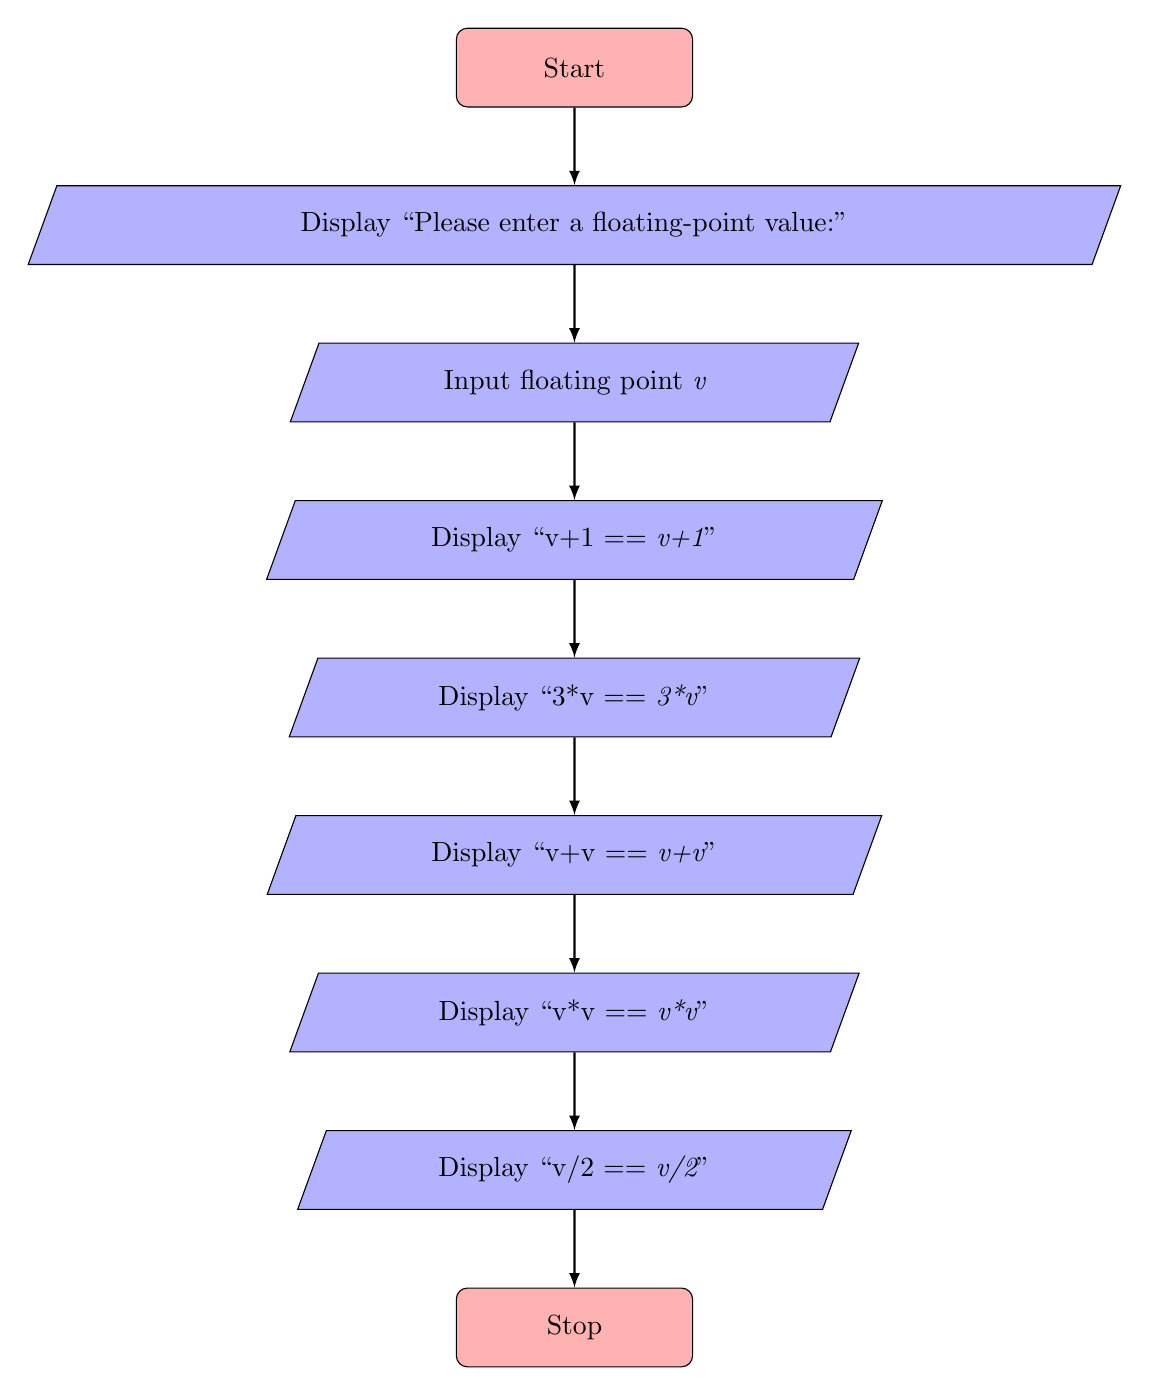
\begin{tikzpicture}[node distance=2cm]

\node (start) [startstop] {Start};
\node (out1) [io, below of=start] {Display ``Please enter a floating-point value:''};
\node (in) [io, below of=out1] {Input floating point {\it v}};
\node (out2) [io, below of=in] {Display ``v+1 == {\it v+1}''};
\node (out3) [io, below of=out2] {Display ``3*v == {\it 3*v}''};
\node (out4) [io, below of=out3] {Display ``v+v == {\it v+v}''};
\node (out5) [io, below of=out4] {Display ``v*v == {\it v*v}''};
\node (out6) [io, below of=out5] {Display ``v/2 == {\it v/2}''};
\node (stop) [startstop, below of=out6] {Stop};

\draw [arrow] (start) -- (out1);
\draw [arrow] (out1) -- (in);
\draw [arrow] (in) -- (out2);
\draw [arrow] (out2) -- (out3);
\draw [arrow] (out3) -- (out4);
\draw [arrow] (out4) -- (out5);
\draw [arrow] (out5) -- (out6);
\draw [arrow] (out6) -- (stop);

\end{tikzpicture}


\end{document}
